% -*- root: article.tex -*-
\subsection{Percepção dos Desenvolvedores}
Analisamos a percepção dos desenvolvedores sobre as 4 más práticas de alta recorrência. As Figuras \ref{fig:lcui} e \ref{fig:all-resources} apresentam gráficos de violino da percepção dos desenvolvedores sobre essas más práticas. No eixo y, 0 (zero) indica códigos não percebidas pelos desenvolvedores como problemáticas (ou seja, responder \emph{não} à pergunta: este código apresenta algum problema de design e/ou implementação?), enquanto valores de 1 a 5 indicam o nível de severidade para o problema percebido pelo desenvolvedor.

\begin{figure}
	\centering
	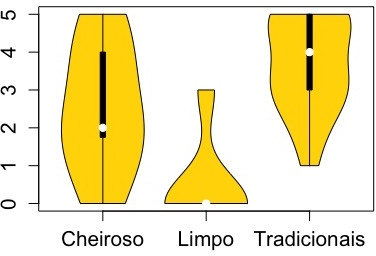
\includegraphics[width=0.3\textwidth]{plot-lcui-violin2.jpg}
	\caption{LCUI}
	\label{fig:lcui}
\end{figure}

Na Figura \ref{fig:lcui} comparamos classes Android afetadas pela má prática LCUI de classes limpas e classes afetadas por maus cheiros tradicionais. Notamos que, desenvolvedores de fato percebem classes afetadas pela má prática LCUI como problemáticas (p-value 0.005921 e $\delta$ 0.6875 (large)). Bem como, classes afetadas por maus cheiros tradicionais também são percebidas como problemáticas (p-value 2.125e-05 e $\delta$ -0.8947368 (large)). Porém, não podemos afirmar se, maus cheiros tradicionais são considerados mais ou menos importantes do que a má prática LCUI (p-value 0.07681 e $\delta$ -0.4342105 (medium)). Ao observar as respostas abertas, a maioria dos participantes pontuou a questão de haver lógica na classe de \textit{front-end}, que é o ponto central desta má prática, como o problema. Podemos citar S2P11 que diz ``\textit{[...] Não há nenhuma arquitetura implementada, o que causa a classe fazendo muito mais do que é de sua alçada. O método onListItemClick está muito complexo, contendo 7 condições [...]}''.

A Figura \ref{fig:all-resources} reúne 4 diferentes pares de gráficos violinos. O primeiro compara recusos afetados por quaisquer das 3 más práticas (LPA, RM e NRD) com recursos limpos. O segundo, terceiro e quarto, distrincha cada má prática individualmente, ou seja, recursos afetadas por aquela má prática em comparação com recursos limpos. 

Com base na Figura \ref{fig:resources} podemos observar que, de fato, desenvolvedores percebem, de forma geral, recursos afetados pelas más práticas LPA, RM ou NRD, como problemáticos (p-value 0.007986 e $\delta$ 0.4335664 (medium)). 

Entretando, ao analisar cada má prática individualmente, vemos na Figura \ref{fig:lpa} que, desenvolvedores de fato percebem recursos afetados pela má prática LPA como problemáticos (p-value 0.02231 e $\delta$ 0.8571429 (large)). Na \ref{fig:rm}, com relação a má prática RM, apesar de haver alguma percepção, estatísticamente ela não é significativa (p-value 0.3433). Na Figura \ref{fig:nrd}, com relação a má prática NRD, não obtivemos dados suficientes para chegar a uma conclusão. 

\begin{figure*}
\centering
\begin{subfigure}{.23\textwidth}
  \centering
  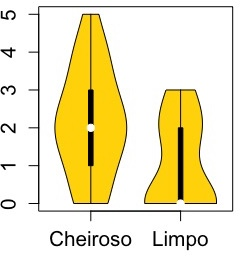
\includegraphics[width=.8\textwidth]{plot-recursos-violin2.jpg}
  \caption{Integrados}
  \label{fig:resources}
\end{subfigure}%
\begin{subfigure}{.23\textwidth}
  \centering
  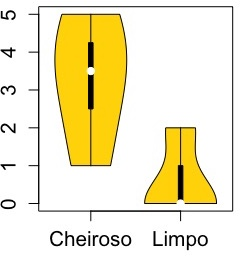
\includegraphics[width=.8\textwidth]{plot-lpa-violin.jpg}
  \caption{LPA}
  \label{fig:lpa}
\end{subfigure}% 
\begin{subfigure}{.23\textwidth}
  \centering
  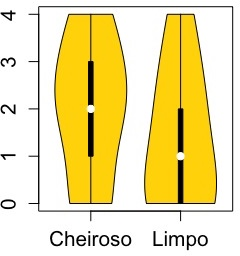
\includegraphics[width=.8\textwidth]{plot-rm-violin.jpg}
  \caption{RM}
  \label{fig:rm}
\end{subfigure}
\begin{subfigure}{.23\textwidth}
  \centering
  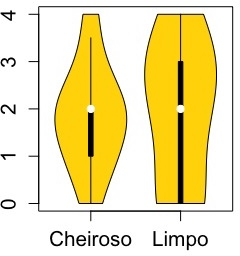
\includegraphics[width=.8\textwidth]{plot-nrd-violin.jpg}
  \caption{NRD}
  \label{fig:nrd}
\end{subfigure}% 
\caption{Gráficos violinos individuais das más práticas que afetam recursos (LPA, RM e NRD).}
\label{fig:all-resources}
\end{figure*}











